% Rewritten from H2Oplus commit c227421700fb7a0a7d808d4c887a877013c553a3,
% referenced by sumo-rl/berth. Layout follows bare_jrnl_new_sample4.tex.
% letterpaper is the valid IEEEtran option for the supplied letter-size layout.
\documentclass[letterpaper,journal]{IEEEtran}
\pdfminorversion=7
\usepackage[T1]{fontenc}
\usepackage{amsmath,amssymb,amsfonts}
\usepackage{array,booktabs}
\usepackage{graphicx}
\usepackage{cite}
\usepackage{url}
\usepackage{microtype}
\usepackage[hidelinks]{hyperref}
\hypersetup{
 pdftitle={Completion-Aware Bus Holding Using Hybrid Offline and Simulation-Based Reinforcement Learning},
 pdfauthor={Yifan Zhang, Liang Zheng, Qifan Zhang},
 pdfsubject={Bus holding, passenger time, and journey completion},
 pdfkeywords={public transportation, bus holding, hybrid reinforcement learning}
}
\hyphenation{rein-force-ment micro-simu-la-tion}
\newcommand{\E}{\mathbb{E}}
\newcommand{\ind}{\mathbb{I}}
\newcommand{\clip}{\operatorname{clip}}
\newcommand{\sigmoid}{\operatorname{sigmoid}}
\newcommand{\Qmin}{\overline{Q}_{\min}}
\newcommand{\Rcmp}{R_{\mathrm{cmp}}}
\newcommand{\Ndep}{N_{\mathrm{dep}}}
\newcommand{\Ncmp}{N_{\mathrm{cmp}}}
\newcommand{\hmax}{h_{\max}}
\newcommand{\hbase}{h_{\mathrm{base}}}
\newcommand{\hfinal}{h_{\mathrm{final}}}
\newcommand{\hrefctrl}{h_{\mathrm{ref}}}

\begin{document}
\title{Completion-Aware Bus Holding Using Hybrid Offline and Simulation-Based Reinforcement Learning}
\author{Yifan Zhang, Liang Zheng, and Qifan Zhang%
\thanks{Yifan Zhang and Liang Zheng are with Central South University, Changsha, Hunan, China (e-mail: erzhu419@gmail.com; 204201048@csu.edu.cn; zhengliang@csu.edu.cn).}%
\thanks{Qifan Zhang is with the Faculty of Information Technology, Monash University Malaysia, Malaysia (e-mail: zhangqifan0419@gmail.com).}}
\markboth{Manuscript Prepared for IEEE Transactions on Intelligent Transportation Systems}%
{Zhang \MakeLowercase{\textit{et al.}}: Completion-Aware Bus Holding}
\maketitle

\begin{abstract}
Learning a bus holding policy in a fast simulator avoids exploratory control of an operating fleet, but reducing passenger time alone can leave more journeys unfinished. We develop a completion-aware controller that combines logged microscopic simulation data with further learning in a calibrated event-based simulator. A shared policy chooses additional holding times for 12 directional services. It represents zero hold explicitly and learns from an exact accounting of waiting and in-vehicle time. A simple execution rule keeps a lightly loaded bus at a stop for 60 seconds when passenger arrivals continue and no following bus is active, within a specified part of the service horizon. We test this controller against an otherwise identical controller with a shorter rule active over a narrower time window. Evaluation covers 1,350 fresh microscopic simulation episodes; the primary comparison uses ten independent environment blocks, three demand levels, and five trained policies. The extended rule reduces generalized passenger time from 2,484.86 to 2,392.73 seconds per passenger who starts a journey, a 3.71\% reduction. Average waiting time falls by 56.23 seconds, while in-vehicle time rises by 20.34 seconds. Journey completion increases from 96.185\% to 96.650\%. Both prespecified criteria are met in all ten blocks. These results support the rule's added benefit for the tested learned controller and make its passenger tradeoff explicit.
\end{abstract}
\begin{IEEEkeywords}
Optimization and control, data-based approaches, public transportation, road transportation, bus holding, hybrid reinforcement learning.
\end{IEEEkeywords}

\section{Introduction}
\label{sec:introduction}
\IEEEPARstart{A}{ bus} delayed on a busy route encounters more waiting passengers and spends longer serving them. The following bus then encounters fewer passengers and catches up. This feedback can turn a small delay into a long gap followed by several buses arriving together \cite{rezazada2024review,daganzo2009headway}. Holding a bus at a stop can restore spacing and reduce waiting downstream, but it also delays people already on board. A useful controller must balance these costs and preserve passengers' opportunities to complete their journeys \cite{delgado2012holding}.

Reinforcement learning (RL) offers a way to make these decisions from traffic, headway, and passenger information. Existing studies have considered dynamic holding, asynchronous decisions, and interactions between services sharing a corridor \cite{alesiani2018reinforcement,wang2020real,wang2021asynchronous,wang2023multiobjective}. Their practical use raises a familiar question: where should a policy acquire its experience? Exploratory actions on an operating fleet affect passengers directly. Logged data avoid this problem but provide limited coverage of alternative actions. A fast simulator supplies additional experience, although its travel times, boarding processes, and service interactions may differ from those in the target environment.

Hybrid Offline-and-Online (H2O) RL addresses this setting by combining a fixed target-domain dataset with interaction in a different simulator \cite{niu2022h2o}. H2O+ extends the approach to different offline and online learners \cite{niu2025h2oplus}. We adapt this framework to bus holding using microscopic simulation records for offline learning and a calibrated event-based model for further training. All online interaction during training occurs in the latter model. The evaluation target is also a simulator; no operating fleet is used for exploration or testing.

A second problem concerns the objective itself. Over a fixed service horizon, a controller can lower accrued passenger time while leaving more journeys unfinished. Keeping a lightly loaded bus moving may benefit its current passengers yet remove a boarding opportunity for people arriving shortly afterward. Their waiting time is counted until the horizon, but the rest of an unfinished journey lies outside that accounting period. During development, improvements in the time objective sometimes coincided with unacceptable reductions in completion.

We therefore combine the learned policy with an explicit passenger-service rule. After ordinary boarding and alighting, a lightly loaded bus waits for 60~s if a preceding bus has served the stop, no following bus is active, and the current eligible arrival rate is positive. The rule applies only during a fixed part of the service horizon. Its purpose is to retain a boarding opportunity where the learned time objective alone may provide insufficient protection.

The study develops a shared, event-based holding controller with an explicit zero-hold action and passenger-time accounting across simultaneous requests. It combines hybrid offline and simulator-based learning with a transparent rule for retaining boarding opportunities. A matched evaluation then tests whether extending this rule reduces passenger time while preserving journey completion.

The central comparison holds the trained policy parameters and prior action calibration fixed. It changes an earlier 20-s rule, active during a narrower window, to the 60-s rule active over a wider window. Across ten independent test blocks, generalized passenger time falls by 92.12~s per departed passenger and completion rises by 0.466 percentage points on average. A decomposition shows the practical tradeoff: less waiting outweighs additional time on board.

\section{Related Work}
\label{sec:related}
\subsection{Bus Holding and Passenger Service}
Classical bus control uses headway or schedule information to limit the propagation of disturbances. Daganzo \cite{daganzo2009headway} analyzes headway-based holding, whereas Xuan \emph{et al.} \cite{xuan2011dynamic} study schedule reliability through dynamic linear control. Passenger-oriented optimization explicitly weighs waiting against additional time on board \cite{delgado2012holding}. Real-time methods incorporate changing running times and demand \cite{sanchezmartinez2016realtime}, and predictive control uses forecasts of headway evolution to choose holding actions \cite{andres2017predictive}.

RL has extended this line of work to more complex operational states. Alesiani and Gkiotsalitis \cite{alesiani2018reinforcement} study high-frequency holding, and Wang and Sun \cite{wang2020real} develop a multi-agent controller. Later work handles asynchronous decisions \cite{wang2021asynchronous}, multiline services sharing a corridor \cite{wang2023multiobjective}, and robustness through distributional multi-agent learning \cite{wang2023robust}. These studies already establish asynchronous and coordinated bus control as active research topics. Our contribution concerns how a hybrid-learned policy is represented, executed, and evaluated when both passenger time and finite-horizon completion matter.

\subsection{Learning from Offline Data and Further Interaction}
Soft actor-critic (SAC) learns an entropy-regularized policy from replayed interactions \cite{haarnoja2018soft,haarnoja2018applications}. Offline methods address the difficulty of evaluating actions poorly represented in a fixed dataset. Conservative Q-learning lowers estimates for unsupported actions \cite{kumar2020cql}, while implicit Q-learning (IQL) learns an expectile value and extracts a policy by advantage-weighted regression \cite{kostrikov2022iql}. We use IQL for initialization and SAC-style objectives during simulator training.

Continuing an offline policy can be unstable because the replay distribution and value estimates change. Balanced replay and critic ensembles \cite{lee2022balanced}, value calibration \cite{nakamoto2023calql}, and policy expansion \cite{zhang2023pex} provide different responses. Reinforcement learning with prior data mixes existing and newly collected experience \cite{ball2023efficient}; warm-start RL instead uses a short initialization period before continuing without offline replay \cite{zhou2025wsrl}. We retain offline replay and gradually release actor updates. These choices adapt existing learning ideas to the present control setting.

Offline training followed by online refinement has also been explored for coordinating ride-pooling and public transit \cite{hu2025rgcql}. Consequently, the present study does not claim to introduce offline-to-online learning to transportation. Its focus is fixed-route holding with asynchronous stop events, a separate training simulator, and an explicit completion rule.

\subsection{Learning across Simulator Dynamics}
Off-dynamics RL estimates a conditional dynamics ratio using domain classifiers and uses it to correct rewards \cite{eysenbach2021off}. H2O and H2O+ combine target-domain records with simulation while accounting for differences in dynamics \cite{niu2022h2o,niu2025h2oplus}. Such correction is useful only if the estimated quantities generalize beyond the training trajectories.

We retain H2O+'s mixed-data value-learning structure but assign equal weights to simulator transitions. The domain classifiers did not generalize adequately to held-out trajectories and are used only to diagnose the dynamics mismatch. Section~\ref{sec:method} describes this choice and its empirical basis.

\section{Bus Holding Problem}
\label{sec:problem}
\subsection{Decisions, Observations, and Actions}
One shared policy controls 12 directional services over a horizon of \(T=24{,}000\)~s. A decision is requested at a nonterminal stop after the bus completes its mandatory boarding and alighting service. The action specifies additional holding only. During that hold, later arrivals may board if capacity remains.

Several buses may request control at the same physical time. We order these requests by service and vehicle identifier, choose their actions sequentially, and advance the simulator only after the full group has been processed. At each step, the policy sees the pending requests and actions already selected for the group. This event-based representation has variable transition durations, as in a semi-Markov decision process \cite{sutton1999between}.

The observation contains five group-level variables and up to 16 padded event records, or slots. The group-level variables are the current time, number of requests, position of the current request, and total waiting and onboard passenger counts. A slot describes the service and stop, forward and backward headways and their scheduled targets, eligible waiting passengers, onboard load, eligible passenger-arrival rate, base service time, and indicators of the preceding and following buses. Passenger quantities are normalized using capacity. Each normalized slot contains an activity flag, 12 local features, and the previously selected action, giving \(5+16(14)=229\) inputs. Inactive slots are masked. We denote this encoded observation at decision \(k\) by \(s_k\), a generic such state by \(s\), and its successor by \(s'\). This compact observation omits parts of the traffic and passenger histories; its Markov sufficiency is an assumption.

Let \(a_k\in[-1,1]\) be the normalized action at decision \(k\). The additional hold is
\begin{equation}
 h_k=\frac{a_k+1}{2}\hmax,\qquad \hmax=60~\mathrm{s}.
 \label{eq:action}
\end{equation}
Thus \(a_k=-1\) is exact zero hold; \(a\) denotes a generic normalized action below. The cap concerns additional holding and does not replace mandatory passenger service.

\subsection{Passenger-Time Objective}
Let \(t_k\) be the physical time of decision \(k\), and let \(\Delta t_k\) be the elapsed time until the next decision. Within a simultaneous group, intermediate transitions have \(\Delta t_k=0\). Only its last transition carries the interval to the next physical event or the horizon.

Denote the numbers of waiting and onboard passengers at time \(u\) by \(N_{\mathrm{w}}(u)\) and \(N_{\mathrm{v}}(u)\). The physical reward is the negative accrued generalized passenger time,
\begin{equation}
 r_k=-\int_{t_k}^{t_k+\Delta t_k}
       [2N_{\mathrm{w}}(u)+N_{\mathrm{v}}(u)]\,\mathrm{d}u .
 \label{eq:reward}
\end{equation}
Waiting time receives weight two and in-vehicle time weight one. Zero-duration transitions have zero reward. Since positive-duration intervals do not overlap, summing their costs counts each waiting or in-vehicle passenger-second once. The initial interval before any controllable event is policy independent and is added when evaluating the full horizon.

The return formed from (\ref{eq:reward}) is undiscounted. Let \(z_k\in\{0,1\}\) equal one when transition \(k\) ends the episode. The Bellman continuation is \(1-z_k\); no extra discount is applied for the duration between events. The learning objective is to maximize expected return in the microscopic target environment, using a fixed offline dataset and a limited number of interactions in the faster training simulator.

For evaluation, let \(\Ndep\) count all passengers who start their journeys and \(\Ncmp\) count those who finish by \(T\). We report
\begin{align}
 W&=\frac{1}{\Ndep}\int_0^T N_{\mathrm{w}}(u)\,\mathrm{d}u,\qquad
 V=\frac{1}{\Ndep}\int_0^T N_{\mathrm{v}}(u)\,\mathrm{d}u,
 \label{eq:times}\\
 Y&=2W+V,\qquad
 \Rcmp=\frac{\Ncmp}{\Ndep},\qquad
 U=\Ndep-\Ncmp .
 \label{eq:endpoints}
\end{align}
In (\ref{eq:times}), \(W\) and \(V\) are accrued waiting and in-vehicle seconds per departed passenger. In (\ref{eq:endpoints}), \(Y\) is generalized seconds per departed passenger, \(\Rcmp\) is the journey-completion rate, and \(U\) is the unfinished-passenger count. The denominator includes passengers whose journeys remain unfinished. Their accrued waiting and in-vehicle time also remain in the numerator; time beyond \(T\) is not observed.

Within a fixed demand realization, minimizing \(Y\) and maximizing the physical return give the same policy ordering. Across different demand levels, the total-cost training objective and the equally averaged per-passenger evaluation need not give the same weights to each scenario. Completion is measured separately because a low accrued-time objective does not guarantee that journeys finish.

\subsection{Offline Records and Training Simulator}
The offline dataset contains tuples \((s_k,a_k,r_k,s_{k+1},\Delta t_k,z_k)\) from the microscopic Simulation of Urban MObility (SUMO) environment \cite{lopez2018microscopic}. The learner adds experience only from a calibrated event-based simulator. Both environments share service routes, stop sequences, timetables, capacities, passenger journeys, and the observation, action, and reward definitions above.

The event-based model uses calibrated segment running times and boarding processes in place of microscopic road traffic. Passenger transfers are released after the preceding leg actually finishes, so a later leg cannot be boarded before the passenger reaches it. Matching these operational definitions allows replay to be combined, but does not make the two environments' transition dynamics identical. Their response agreement is checked before policy evaluation, as described in Section~\ref{sec:design}.

\section{Learning and Execution}
\label{sec:method}
Fig.~\ref{fig:overview} separates learning from execution. The learner produces a holding proposal. Two deterministic operations then calibrate its duration and apply the completion rule. All parameters are fixed during target evaluation.

\begin{figure*}[!t]
\centering
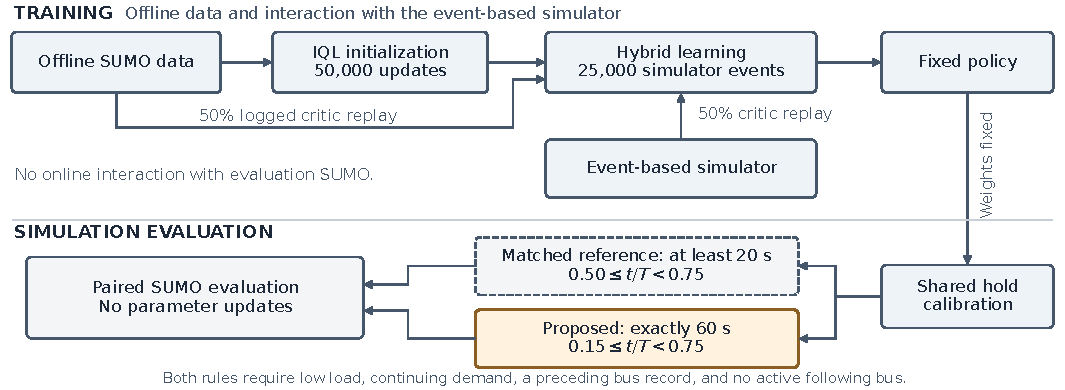
\includegraphics[width=\textwidth]{figures/controller_overview.pdf}
\caption{Learning and evaluation of the bus holding controller. Offline microscopic records and further interaction in an event-based simulator produce a fixed actor. The primary comparison uses that same actor and hold calibration in both controllers, changing the completion rule's duration and activation window. Target evaluation supplies no training updates.}
\label{fig:overview}
\end{figure*}

\subsection{Representing Exact Zero Hold}
The actor, critic, and value networks use separate structured encoders. A shared network maps each event slot to 128 features. The current slot, active-slot mean and maximum, earlier-slot mean, and later-slot mean are combined with the group-level variables to obtain a 256-feature representation. The heads then use two hidden layers of 256 units. There are two critic heads and their target copies.

Exact zero hold is common and operationally distinct from a small positive hold. We therefore use a hurdle policy: a binary decision determines whether to hold, and a continuous distribution determines the positive duration. Let \(\pi_\phi\) denote this policy, with actor parameters \(\phi\), holding probability \(p_\phi(s)\), latent normal mean \(\mu_\phi(s)\), and positive standard deviation \(\sigma_\phi(s)\). With \(\sigmoid(x)=1/(1+e^{-x})\), its normalized action is generated by
\begin{equation}
\begin{aligned}
 a&=-1 &&\text{with probability }1-p_\phi(s),\\
 a&=2\sigmoid(\zeta)-1 &&\text{otherwise},\\
 \zeta&\sim\mathcal{N}(\mu_\phi(s),\sigma_\phi^2(s)).
\end{aligned}
\label{eq:hurdle}
\end{equation}
Here \(\zeta\) is the latent normal variable. The positive branch in (\ref{eq:hurdle}) has density
\begin{equation}
 f_\phi(a\mid s)=
 \frac{2\,\mathcal{N}\!\left(\log\frac{1+a}{1-a};
                 \mu_\phi(s),\sigma_\phi^2(s)\right)}{1-a^2},
 \quad -1<a<1 .
 \label{eq:density}
\end{equation}
In (\ref{eq:density}), \(\mathcal{N}(x;\mu,\sigma^2)\) denotes the normal density evaluated at \(x\), and the Jacobian follows directly from the logistic transformation. Likelihoods use the point mass at \(-1\) together with the continuous density on \((-1,1)\). We write the density with respect to this common point-mass-plus-Lebesgue measure as \(q_\phi(a\mid s)\): it equals \(1-p_\phi(s)\) at zero hold and \(p_\phi(s)f_\phi(a\mid s)\) on the positive branch. Positive actions are clipped near the numerical endpoints when evaluating likelihoods, including logged maximum holds; stored actions and physical holds are unchanged by this likelihood calculation.

Evaluation is deterministic: if \(p_\phi(s)<0.5\), the proposal is \(h_\phi(s)=0\); otherwise it is \(h_\phi(s)=\hmax\sigmoid(\mu_\phi(s))\), using the action-to-hold map in (\ref{eq:action}). The latter is the positive branch's median hold, which generally differs from its mean.

\subsection{Offline Initialization and Simulator Learning}
Five actors are initialized with 50,000 IQL updates \cite{kostrikov2022iql}. Let \(\mathcal D_{\mathrm{off}}\) and \(\mathcal D_{\mathrm{sim}}\) denote the empirical sampling distributions of offline and simulator replay. We write \(\E\) for expectation and \(\ind\) for the indicator of a stated condition. Let \(\Qmin(s,a)\) be the minimum of the two target critics and \(V_\nu(s)\) the expectile value with parameters \(\nu\). Rewards are multiplied by \(\kappa=10^{-4}\) inside the trainer for numerical conditioning; the stored data and reported outcomes retain physical units. All critics and values below use these scaled rewards. For \(A(s,a)=\Qmin(s,a)-V_\nu(s)\), the value minimizes the expectile loss
\begin{equation}
 L_V=\E_{\mathcal D_{\mathrm{off}}}
       [\,|0.7-\ind\{A<0\}|A^2\,].
 \label{eq:value}
\end{equation}
With \(A=A(s,a)\), the actor minimizes the negative logged-action likelihood with weight
\begin{equation}
\begin{aligned}
 w(A)&=\min\{\exp(3A),100\},\\
 L_{\pi,\mathrm{off}}&=-\E_{\mathcal D_{\mathrm{off}}}
                 [w(A)\log q_\phi(a\mid s)] .
\end{aligned}
 \label{eq:iql}
\end{equation}
Here \(L_V\) in (\ref{eq:value}) is the value-fitting loss, \(w(A)\) is the capped regression weight, and \(L_{\pi,\mathrm{off}}\) in (\ref{eq:iql}) is the offline actor loss.

The initialized policy first collects 5,000 simulator events without learning. Subsequent critic minibatches combine offline and simulator transitions equally. Following the H2O+ mixed-backup construction \cite{niu2025h2oplus}, define the soft bootstrap \(B_{\mathrm{soft}}\) and critic target \(y_k\), with entropy temperature \(\alpha>0\), by
\begin{align}
 B_{\mathrm{soft}}(s')&=\E_{a'\sim\pi_\phi(\cdot\mid s')}
       [\Qmin(s',a')-\alpha\log q_\phi(a'\mid s')], \label{eq:soft}\\
 y_k&=\kappa r_k+(1-z_k)
          [0.1V_\nu(s_{k+1})+0.9B_{\mathrm{soft}}(s_{k+1})].
 \label{eq:backup}
\end{align}
Here \(a'\) is a successor-state action in (\ref{eq:soft}); \(y_k\) in (\ref{eq:backup}) combines the physical reward with the mixed bootstrap. The critic uses a Huber loss with threshold one. The expectile value continues to be updated from the offline transitions during simulator training. The actor minimizes
\begin{equation}
 L_{\pi,\mathrm{sim}}=\E_{s\sim\mathcal D_{\mathrm{sim}},\,a\sim\pi_\phi(\cdot\mid s)}
       [\alpha\log q_\phi(a\mid s)-Q_{\min}(s,a)],
 \label{eq:sacactor}
\end{equation}
where \(L_{\pi,\mathrm{sim}}\) denotes the simulator-phase actor loss and \(Q_{\min}\) is the minimum of the current critics, distinct from the target-critic minimum \(\Qmin\). The entropy temperature \(\alpha\) is learned with target entropy zero \cite{haarnoja2018soft,haarnoja2018applications}. The binary branch is summed exactly; the positive branch uses one reparameterized sample per state.

Actor updates using (\ref{eq:sacactor}) and temperature updates remain frozen until 10,000 simulator events. The actor learning-rate multiplier increases from approximately 0.1 to 1.0 over events 10,000--15,000, then decreases linearly to 0.25 over events 15,000--25,000. After each actor update, parameter interpolation with coefficient \(5\times10^{-5}\) pulls the actor toward its own 10,000-event parameters. This limits drift while the critics adapt. Temperature updates resume at their nominal rate.

Table~\ref{tab:training} gives the remaining settings. Each policy receives 50,000 updates from offline data and 20,000 updates during simulator training. The nominal simulator budget is 25,000 events; two of the five runs end at 24,999 to avoid splitting a simultaneous decision group. We use only the final scheduled checkpoint, without selecting among checkpoints on target outcomes.

\begin{table}[!t]
\caption{Training Settings}
\label{tab:training}
\centering
\footnotesize
\begin{tabular}{@{}p{0.58\columnwidth}p{0.36\columnwidth}@{}}
\toprule
Setting & Value\\
\midrule
Slot / fused representation & 128 / 256\\
Hidden layers in each head & \(256,256\)\\
Critic / actor batch size & 256 / 128\\
Offline fraction of critic batch & 0.5\\
Adam learning rate & \(3\times10^{-4}\)\\
Target-network update rate & 0.005\\
Log standard deviation bounds & \([-5,2]\)\\
Initial entropy temperature & 1.0\\
Reward multiplier & \(10^{-4}\)\\
IQL expectile / weight cap & 0.7 / 100\\
Offline / simulator-training updates & 50,000 / 20,000\\
Nominal simulator-event budget & 25,000\\
Independent training seeds & 5\\
\bottomrule
\end{tabular}
\end{table}

\subsection{Handling Unreliable Dynamics Weights}
Joint classifiers observe \((s,a,s',\Delta t/T)\), and marginal classifiers observe \((s,a)\). Their logit difference is intended to estimate the log conditional dynamics ratio between logged microscopic and training-simulator transitions \cite{eysenbach2021off,niu2025h2oplus}. Validation holds out complete trajectories rather than randomly splitting correlated rows.

The mean joint classification area under the receiver-operating characteristic curve is 0.9477 on training data but 0.4520 on held-out data. The mean raw importance-weight effective sample size is only 6.15\% of the validation sample. The final learner therefore assigns unit weights to simulator critic losses. The classifiers remain diagnostic and do not alter the updates in (\ref{eq:backup}). We refer to this learner as H2O+-based to identify its mixed-data construction while making this implementation choice explicit.

\subsection{Calibrating the Holding Proposal}
At physical time \(t\), let \(\rho=t/T\) denote the horizon fraction. Denote forward and backward headways by \(H_f,H_b\), and their scheduled targets by \(H_f^*,H_b^*\), all in seconds. The indicator \(I_f=1\) means that the preceding scheduled bus has completed base service at this stop. The indicator \(I_b=1\) means that the following scheduled bus is currently active. An inactive follower can still be scheduled to depart later.

The headway-based duration is
\begin{equation}
 h_H(s)=\clip\left(
 \frac{I_b(H_b-H_b^*)-I_f(H_f-H_f^*)}{2},\,0,\,60
 \right).
 \label{eq:headway}
\end{equation}
The calibrated proposal is
\begin{equation}
 \hbase(s)=
 \begin{cases}
 \min\{h_\phi(s),\max[h_\phi(s)/8,h_H(s)]\},&\rho<0.75,\\
 h_\phi(s)/8,&\rho\geq0.75.
 \end{cases}
 \label{eq:calibration}
\end{equation}
In (\ref{eq:headway}), \(\clip(\cdot,0,60)\) truncates its argument to \([0,60]\)~s. The calibrated proposal in (\ref{eq:calibration}) reduces excessive learned holding while retaining a headway response during the first three quarters of the horizon. These fixed choices were made during development and are shared by the two controllers in the main comparison.

\subsection{Completion Rule and Matched Reference}
Let \(n_{\mathrm{on}}\) be the onboard passenger count, \(c>0\) the bus capacity, and \(\lambda\) the current eligible passenger-arrival rate in passengers per second. The rate is obtained from hourly origin--destination demand and scheduled service frequencies, rather than a learned forecast. For horizon-fraction bounds \(0\leq\rho_{\mathrm{lo}}<\rho_{\mathrm{hi}}\leq1\), define
\begin{equation}
\begin{split}
 G_{[\rho_{\mathrm{lo}},\rho_{\mathrm{hi}})}(s)={}&
 \ind\{\rho_{\mathrm{lo}}\leq\rho<\rho_{\mathrm{hi}},\ I_f=1,\ I_b=0\}\\
 &{}\times\ind\{\lambda>0,\ c>0,\ n_{\mathrm{on}}/c\leq0.25\}.
\end{split}
 \label{eq:guard}
\end{equation}
The binary guard in (\ref{eq:guard}) selects the states where the completion rule applies. The completion-aware controller executes
\begin{equation}
 \hfinal(s)=
 \begin{cases}
 60,&G_{[0.15,0.75)}(s)=1,\\
 \hbase(s),&\text{otherwise}.
 \end{cases}
 \label{eq:final}
\end{equation}
Thus the rule applies between 3,600 and 18,000~s. It leaves a lightly loaded bus available for arriving passengers when no following vehicle is active. The 60-s bound limits the added action; it does not guarantee that every journey will finish.

The matched reference uses the identical actor and calibration but retains the earlier service rule,
\begin{equation}
 \hrefctrl(s)=
 \begin{cases}
 \max\{\hbase(s),20\},&G_{[0.50,0.75)}(s)=1,\\
 \hbase(s),&\text{otherwise}.
 \end{cases}
 \label{eq:reference}
\end{equation}
This reference already includes a service rule, so the comparison measures the added effect beyond that rule. It changes both the activation window and the holding floor, testing the complete rule change rather than identifying the separate effect of either parameter.

Controller design used a development set, with some scenarios reused across iterations. Before final evaluation, we fixed both controllers, all five trained policies, the test scenarios, the outcome measures, and the statistical analysis. The final test set was used only for evaluation.

\section{Experimental Design}
\label{sec:design}
\subsection{Network, Data, and Independent Test Blocks}
The benchmark is a simulated urban bus network with 12 directional services for routes 7, 102, 122, 311, 406, and 705 (Fig.~\ref{fig:network}). Every 24,000-s episode has 389 scheduled vehicle trips. Demand multipliers are 0.75, 1.00, and 1.25. Passenger journey-start times receive independent uniform perturbations of at most 120~s, clipped to each source route's original departure-time support. The road network, bus timetable, capacities, and social traffic remain fixed.

\begin{figure}[!t]
\centering
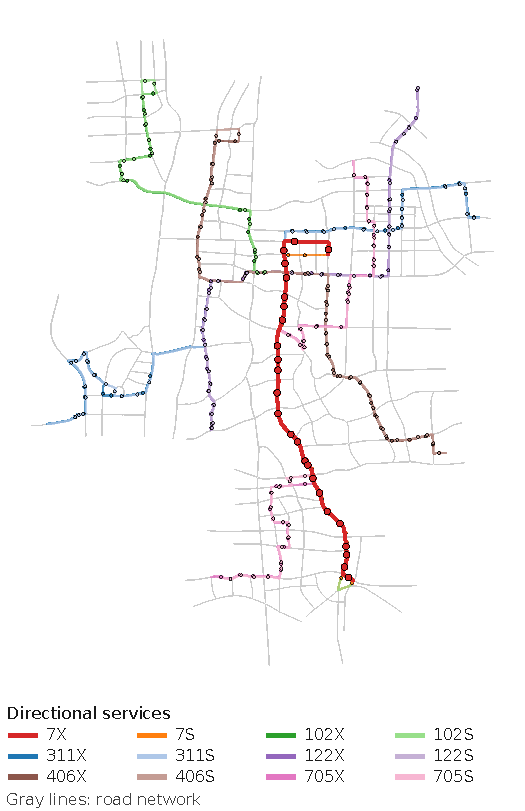
\includegraphics[width=\columnwidth]{figures/network_topology.pdf}
\caption{Road network and 12 directional services in the benchmark. The thicker route is highlighted for visibility; the controller acts on all services. Microscopic and event-based environments use the same route and stop definitions.}
\label{fig:network}
\end{figure}

Offline collection crosses ten environment blocks, three demand levels, and eight behavior policies, yielding 240 complete episodes and 3,284,718 transitions. The behaviors comprise zero hold, two random hurdle policies, four fixed-gain schedule-adjusted headway policies, and a myopic passenger-time policy. They provide varied actions and are not assumed to be experts. The replay contains 240 terminal records and 1,025,206 zero-duration transitions. Across all 240 episodes, the recorded rewards and passenger-time integrals give the same total cost.

For final evaluation, ten new environment blocks are crossed with three demand levels and five actor seeds. A block uses one demand-realization seed and one microscopic-traffic seed shared across its demand levels. These ten blocks are disjoint from training and development. Within each block and demand level, all controllers encounter the same external conditions.

Nine controllers are evaluated, producing \(10\times3\times5\times9=1{,}350\) episodes. The primary comparison comprises the 300 episodes from (\ref{eq:final}) and (\ref{eq:reference}), or 150 matched pairs. The remaining seven controllers provide descriptive context. The independent unit for inference is the environment block, not a transition, an actor seed, or an individual episode.

\subsection{Agreement between Training and Target Simulators}
Before final evaluation, the event-based model was compared with microscopic simulation in 30 matched scenarios. Under zero holding, the largest point differences were 4.61\% for generalized passenger time, 8.75\% for waiting time, 1.66\% for in-vehicle time, 0.43 percentage points for completion, and 1.04\% for completed vehicle-trip duration. Prespecified tolerances were 15\% for generalized and waiting time, 10\% for in-vehicle time, 3 percentage points for completion, and 5\% for trip duration. Passenger demand and decision count had separate 3\% and 5\% tolerances.

A second check applied seven nonzero holding interventions to those scenarios and compared their changes from zero hold. The largest absolute endpoints of the 95\% intervals were 0.574 percentage points for completion and 3.90\%, 4.98\%, and 2.00\% for normalized generalized, waiting, and in-vehicle time responses. Time responses are normalized by the corresponding SUMO zero-hold means. Their respective tolerances were 3 percentage points and 10\%. All prespecified response checks passed. The intervals used 10,000 bootstrap resamples of episode quantities within demand levels, sampling the two simulators separately. These checks establish agreement for the tested operating conditions and interventions, rather than for all states a learned policy may visit.

Offline records were collected with SUMO~1.27.1 and Python~3.10.12. Evaluation used SUMO~1.25.0 through libsumo, with Python~3.8.20. Every controller uses the same evaluation runtime. Software-version effects were not evaluated separately.

\subsection{Comparison Controllers}
The primary reference uses the same five trained policies and hold calibration as the proposed controller. Additional comparisons include a transit-adapted H2O+ baseline, online-only SAC, the learned policy without execution rules, and four intermediate training variants. These variants alter the data used for actor updates, the timing of those updates, the learning-rate schedule, and parameter anchoring. Their results are reported descriptively alongside the primary comparison.

The transit-adapted H2O+ control uses active dynamics weights; the final learner and subsequent stabilization variants use unit weights. Online-only SAC has the same nominal simulator-event budget but no 50,000-update offline initialization. Therefore, its training computation is not matched to that of the hybrid learner.

\subsection{Prespecified Statistical Analysis}
For each environment block \(b\), we first average the 15 paired differences from five actor seeds \(j\) and three demand multipliers \(d\):
\begin{equation}
 \Delta Y_b=\frac{1}{15}\sum_{j=1}^{5}
       \sum_{d\in\{0.75,1,1.25\}}
       (Y^{\mathrm{final}}_{bjd}-Y^{\mathrm{ref}}_{bjd}).
 \label{eq:block}
\end{equation}
The same averaging as in (\ref{eq:block}) gives the completion-rate difference \(\Delta R_{\mathrm{cmp},b}\) and unfinished-passenger difference \(\Delta U_b\), always proposed minus reference. Unsubscripted differences denote equal-weight means across the ten blocks. Reported overall means give equal weight to the scenario--actor pairs. They are not obtained by pooling passengers across episodes.

We require both a time benefit and completion noninferiority. A time win is \(\Delta Y_b<0\); a completion win is \(\Delta R_{\mathrm{cmp},b}>-0.003\), using a 0.3-percentage-point noninferiority margin. For \(w\) wins among ten blocks, the one-sided exact sign-test probability is
\begin{equation}
 p(w)=2^{-10}\sum_{\ell=w}^{10}\binom{10}{\ell}.
 \label{eq:sign}
\end{equation}
Here \(\ell\) is a possible win count in the binomial tail in (\ref{eq:sign}), distinct from the decision index \(k\). Ties count as nonwins. Each component uses a significance level of 0.025; at least nine wins are required. The intersection--union decision succeeds only when both components pass. The protocol also requires favorable mean and demand-level directions and a complete evaluation matrix.

The sign test assesses directional consistency across independent blocks. It does not provide a confidence interval for the population mean difference. Demand- and actor-specific summaries, waiting/ride decompositions, and comparisons with the other controllers are descriptive.

\section{Results}
\label{sec:results}
\subsection{Passenger-Time and Completion Outcomes}
Table~\ref{tab:primary} reports the primary comparison. Generalized passenger time decreases from 2,484.86 to 2,392.73~s per departed passenger, a mean paired difference of \(-92.12\)~s and a descriptive relative reduction of 3.71\%. Completion increases by 0.466 percentage points. The mean number of unfinished passengers falls by 77.22 per episode, or 11.78\%.

\begin{table}[!t]
\caption{Primary Comparison on Fresh Test Scenarios}
\label{tab:primary}
\centering
\footnotesize
\setlength{\tabcolsep}{3pt}
\begin{tabular}{@{}lrrr@{}}
\toprule
Outcome & Reference & Proposed & Difference\\
\midrule
Generalized time (s/pax) & 2,484.86 & 2,392.73 & \(-92.12\)\\
Waiting time (s/pax) & 720.12 & 663.88 & \(-56.23\)\\
In-vehicle time (s/pax) & 1,044.63 & 1,064.96 & \(+20.34\)\\
Completion (\%) & 96.185 & 96.650 & \(+0.466\) pp\\
Unfinished (pax/episode) & 655.42 & 578.20 & \(-77.22\)\\
\bottomrule
\end{tabular}
\par\smallskip
\begin{minipage}{\columnwidth}
\footnotesize
Reference: same actor and calibration with a 20-s rule in the later window. Proposed: 60-s rule over the wider window. Time is accrued to the common horizon and divided by all departed passengers. Differences are computed before rounding. The abbreviations pax and pp denote passengers and percentage points, respectively.
\end{minipage}
\end{table}

The decomposition makes the passenger tradeoff explicit. Waiting time falls by 56.23~s per departed passenger, while in-vehicle time rises by 20.34~s. With the fixed waiting-time weight,
\[
 2(-56.23)+20.34\approx-92.12~\mathrm{s}.
\]
The proposed controller therefore improves the weighted outcome while imposing a measurable cost on passengers already in vehicles.

Every environment block has lower generalized time and higher completion (Fig.~\ref{fig:blocks}). Both prespecified sign tests have ten wins and \(p=2^{-10}=0.0009766\). All ten completion differences are positive, so meeting the prespecified criterion does not depend on its allowance for small losses.

\begin{figure*}[!t]
\centering
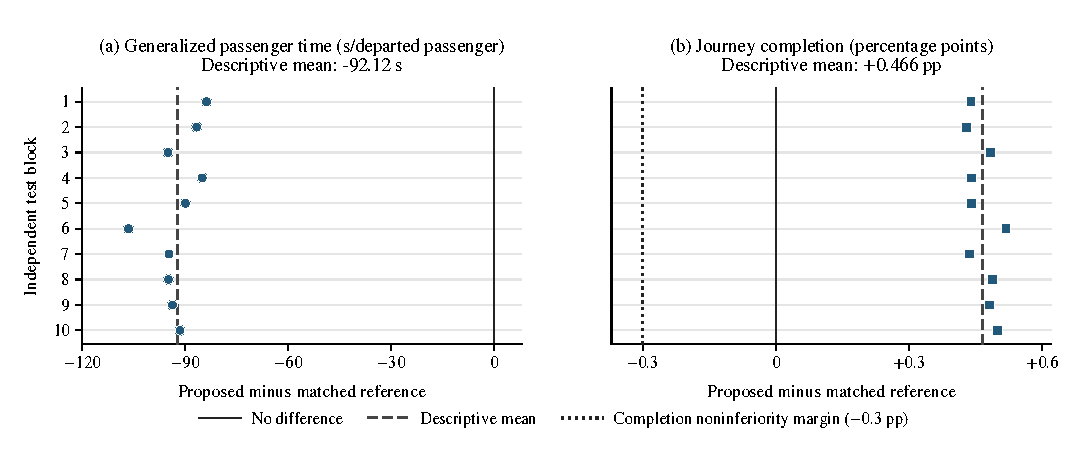
\includegraphics[width=\textwidth]{figures/block_effects.pdf}
\caption{Paired effects in the ten independent test blocks. Each point averages three demand levels and five actor seeds, with proposed minus reference as the difference. Negative generalized time and positive completion are favorable. The completion noninferiority boundary is \(-0.3\) percentage points. Mean lines are descriptive; no confidence interval for the mean is implied.}
\label{fig:blocks}
\end{figure*}

\subsection{Demand and Training-Seed Variation}
The benefit increases with demand (Table~\ref{tab:demand}). At demand multiplier 0.75, generalized time falls by 40.29~s per departed passenger; at 1.25, it falls by 148.46~s. Completion improves at every level. The in-vehicle increase remains close to 20~s across the three levels, while the waiting reduction grows from 30.14 to 84.71~s.

\begin{table}[!t]
\caption{Paired Differences by Demand Level}
\label{tab:demand}
\centering
\footnotesize
\begin{tabular}{@{}lrrr@{}}
\toprule
Demand & \(\Delta Y\) (s/pax) & \(\Delta\Rcmp\) (pp) & \(\Delta U\) (pax)\\
\midrule
0.75 & \(-40.29\) & \(+0.185\) & \(-21.00\)\\
1.00 & \(-87.61\) & \(+0.470\) & \(-70.92\)\\
1.25 & \(-148.46\) & \(+0.741\) & \(-139.74\)\\
\bottomrule
\end{tabular}
\end{table}

The direction also holds for all five trained actors. Their mean time differences range from \(-87.25\) to \(-97.44\)~s, and completion differences range from \(+0.444\) to \(+0.485\) percentage points. These summaries show that the overall direction is not produced by a single training seed.

\subsection{Performance of Other Controllers}
Table~\ref{tab:controls} places the matched result alongside all controllers in the evaluation matrix. The proposed controller has the lowest displayed mean generalized time and the highest completion rate. Its mean generalized time is 201.12~s below online-only SAC and 304.24~s below the transit-adapted H2O+ control.

\begin{table*}[!t]
\caption{Descriptive Outcomes for All Nine Evaluated Controllers}
\label{tab:controls}
\centering
\footnotesize
\begin{tabular}{@{}p{0.25\textwidth}p{0.46\textwidth}rr@{}}
\toprule
Controller & Distinguishing feature & \(Y\) (s/pax) & Completion (\%)\\
\midrule
Completion-aware controller & Final trained policy, hold calibration, and extended completion rule & \textbf{2,392.73} & \textbf{96.650}\\
Matched reference & Same actor and calibration, 20-s later-window rule & 2,484.86 & 96.185\\
Learned policy alone & Final policy without hold calibration or the completion rule & 2,623.19 & 96.453\\
Transit-adapted H2O+ & Hybrid learner with active dynamics weights & 2,696.98 & 96.288\\
Online-only SAC & Simulator learning without offline initialization & 2,593.85 & 96.232\\
Actor updates from simulator data & Actor uses simulator replay after the initial phase & 2,532.20 & 95.894\\
Delayed actor updates & Actor and temperature stay fixed through 10,000 events & 2,569.68 & 96.023\\
Gradual increase in actor learning rate & Adds an actor learning-rate ramp & 2,585.56 & 96.194\\
Actor updates with parameter anchoring & Adds interpolation toward the earlier actor & 2,581.26 & 96.053\\
\bottomrule
\end{tabular}
\par\smallskip
\begin{minipage}{\textwidth}
\footnotesize
Each row averages 150 evaluation episodes. The last four rows are development variants evaluated on the same test scenarios. The prespecified joint test compares the proposed controller with the matched reference. Other rows differ in learning or execution and are descriptive. SAC matches the nominal online-event budget, not the hybrid learner's total update count.
\end{minipage}
\end{table*}

Without hold calibration or the completion rule, the learned policy has a higher completion rate than the matched reference but also higher generalized passenger time. Thus calibration and the earlier rule do not improve every outcome simultaneously. The final rule achieves a better time--completion tradeoff in these scenarios. The other rows change more than one component relative to the proposed controller, so they cannot isolate the contribution of the actor architecture, mixed replay, or stabilization schedule.

\subsection{Action Coverage and Reproducibility}
Zero holding accounts for 80.22\% of offline actions, supporting its explicit representation in the policy. Long holds are much rarer. Within the narrower \([0.50,0.75)\) window used by the reference, 128,437 records satisfy the rule conditions, but only 3.69\% contain holds of at least 30~s. These counts do not describe the wider window used by the proposed controller. The 60-s rule is therefore an explicit operational choice with limited coverage in the offline data.

The released records identify the controller, actor seed, checkpoint, scenario, runtime, and result for each episode. An independent calculation reproduces the primary means, demand and block summaries, and sign-test outcomes. The source code and compact experiment records are available in the project repository.\footnote{\url{https://github.com/erzhu419/sumo-rl/tree/berth}; the bus-control study is in its \texttt{H2Oplus} submodule.} Large replay files, checkpoints, and generated scenario inputs are not included in the repository. Consequently, the public records support checking the reported calculations, while rerunning training also requires the original inputs.

\section{Discussion}
\label{sec:discussion}
\subsection{Why Extra Holding Can Improve Passenger Service}
Holding is usually motivated by restoring headways. Here it also preserves a boarding opportunity. A lightly loaded bus without an active follower can remain at the stop while additional eligible passengers arrive. The rule permits this only during a specified window and at loads no greater than one quarter of capacity. Its benefit is operationally plausible because boarding remains possible during the additional hold.

The waiting/ride decomposition supports that interpretation: all ten blocks show less waiting and more in-vehicle time, with a favorable weighted total. The larger waiting reduction at higher demand is also consistent with more passengers benefiting from the retained opportunity. However, the aggregate comparison does not identify which particular boarding or transfer events caused the completion gain. It also changes the activation window and hold duration together.

The learned policy still determines proposals outside the rule and contributes through the shared calibration. The completion rule modifies its action only under the specified conditions.

\subsection{What the Evidence Supports}
The independent test scenarios show that extending the completion rule reduces generalized passenger time and meets the prespecified completion criterion for the five fixed policies under the tested operating conditions. The sign test supports consistency across environment blocks; it does not quantify uncertainty in the population-average effect. With only ten blocks, the distribution of effect sizes remains uncertain.

The experiment does not establish which learning components are responsible for the controller's performance or whether the learned policy is necessary. The additional comparisons change multiple components, and online-only SAC receives fewer total learner updates because it lacks offline initialization. Conventional headway control with and without the same completion rule is an important missing comparison. These limitations prevent a general claim of superiority over existing holding methods.

\subsection{Transfer and Operational Limits}
Both the source records and evaluation outcomes are simulated. The event-based training model passes the specified agreement checks, but this does not establish transfer to observed operations, another network, or every policy-induced state distribution. Logged and evaluation SUMO versions also differ. A paired evaluation of the same fixed controllers under both versions would help separate software-version effects from other dynamics differences.

The observation compresses histories and future service availability. In particular, an inactive following bus is not necessarily the last scheduled service. The arrival-rate input is constructed from demand and frequency information, and the rule does not predict terminal shortfall explicitly. Its fixed load threshold and time window may need adjustment for other timetables.

Completion is assessed at a finite horizon, and the reward includes only accrued time. A future controller could model terminal shortfall directly or learn a constrained policy, provided its data cover the relevant states and long holding actions. The current physical cap provides a bounded action, not a general operational safety guarantee. Field evaluation would also need dispatch, driver, accessibility, and connection requirements that are outside this benchmark.

\section{Conclusion}
\label{sec:conclusion}
This paper develops a bus holding controller that learns from microscopic simulation records and further interaction in a faster event-based simulator. A shared policy represents exact zero hold, accounts for passenger time across asynchronous events, and supplies a holding proposal. A deterministic completion rule then preserves selected boarding opportunities for lightly loaded buses without an active follower.

On independent test scenarios, replacing an earlier narrow-window rule with the proposed rule reduces generalized passenger time by 92.12~s per departed passenger and increases completion by 0.466 percentage points. The benefit consists of a 56.23-s waiting reduction and a 20.34-s in-vehicle increase. Both prespecified criteria hold in all ten independent blocks. The study supports this rule change for the tested hybrid-learned controller. Comparisons with conventional holding policies under the same completion rule, followed by operational validation, are needed to assess wider applicability.

\section*{Acknowledgment}
OpenAI ChatGPT assisted with restructuring and rewriting the abstract, Sections~\ref{sec:introduction}--\ref{sec:conclusion}, and figure captions from the existing manuscript, source code, and experiment records, and with preparing the schematic and plots from those records.

% Standard IEEEtran column break balances the final reference page.
\IEEEtriggeratref{16}
\bibliographystyle{IEEEtran}
\bibliography{references}
\end{document}
